
%(BEGIN_QUESTION)
% Copyright 2010, Tony R. Kuphaldt, released under the Creative Commons Attribution License (v 1.0)
% This means you may do almost anything with this work of mine, so long as you give me proper credit

A compressed air system has a leak, and you are part of a group of technicians asked to locate the leak.  A pressure transmitter measuring receiver tank pressure is connected to a trend recorder, offering a way for you monitor tank pressure over time.  Setting up for the leak test, one of the technicians on your team runs the compressor until the receiver tank gauge registers normal (full) pressure, then she shuts off the compressor and begins shutting off all the valves shown (dark) in this P\&ID:

$$\includegraphics[width=15.5cm]{i01553x01.eps}$$

After waiting a few hours, you examine the trend of the receiver tank pressure, shown here:

$$\includegraphics[width=15.5cm]{i01553x02.eps}$$

Another technician on your team sees this trend and exclaims, ``Ah-Ha!!  We know the leak is downstream of a pressure regulator, not upstream!''  Puzzled by this, you ask your teammate to explain.  ``Look at the shape of the trend: a straight line sloping down, followed by a curve asymptotically approaching zero PSI.  If the leak were upstream of a regulator, the whole downward trend would be asymptotic with no straight portions.  If you take the Ideal Gas Law ($PV = nRT$) and express it as a differential equation over time (${dP \over dt} V = {dn \over dt} RT$), you see that the rate of pressure fall ($dP \over dt$) is proportional to the rate of air molecule leakage ($dn \over dt$).''

\vskip 10pt

Explain what your teammate is trying to say, in your own words.  {\it Why} would the location of an air leak in this system make a difference in the {\it shape} of the trend?  Furthermore, what would you do to isolate the location of the leak, now that you know it is downstream of a regulator?

\vfil 

\underbar{file i01553}
\eject
%(END_QUESTION)





%(BEGIN_ANSWER)

This is a graded question -- no answers or hints given!

%(END_ANSWER)





%(BEGIN_NOTES)

A leak downstream of a pressure regulator would leak air at a {\it constant} rate so long as the (regulated) pressure at the leak remained constant, because a constant pressure drop across an orifice is analogous to a constant voltage across a resistance: in both cases the result is a constant flow through the restriction.  This constant flow rate of air through the leak is what makes the receiver tank pressure drop linearly.  It is the same principle as voltage across a charged capacitor, discharging through a current regulator: the voltage's rate of descent to zero ($dV \over dt$) will be constant because both the current ($I$) and the capacitance ($C$) are constant quantities and are related to each other by the formula $I = C {dV \over dt}$.

If the leak were upstream of a regulator, the rate of air leakage would vary with pressure the entire time, resulting in an asymptotic pressure drop the whole time.  In other words, an upstream leak would generate an inverse exponential curve resembling that of voltage in a resistor-capacitor discharge circuit.

\vskip 10pt

To isolate the leak, turn the compressor on again to pump up the receiver tank, then close the regulator supply valves one by one until you see the pressure drop level off.  The pressure should hold steady (slope = 0) when there is no air leakage.

%INDEX% Mathematics, calculus: differentiation
%INDEX% Measurement, pressure: troubleshooting

%(END_NOTES)


